\chapter{Desenvolvimento}
\label{cap:5}

\section{Arquitetura Proposta}
Para atingir o objetivo de desenvolver uma RSSF de baixo custo monterário e baixo consumo elétrico para uso
residencial e em escritório, propõe-se utilizar o transceptor \texttt{nRF24L01+} para a comunicação e modelos de
microcontroladores \texttt{AVR} como unidade controladora dos nós.

A rede será da topologia árvore e terá as três características consideras por
\citeonline{hai_nayak_stojmenovic2010} citadas anteriormente: sob demanda para os nós que possuem atuadores;
períodica para os sensores em geral; e orientada à eventos para sensores considerados críticos, como o de gás.

Cada nó da rede poderá comportar até 2 sensores ou atuadores. Isso é útil pois existem alguns dispositivos que
normalmente atuam em conjunto como o sensor de temperatura com o de umidade ou o sensor de tensão com um relé
eletromecânico em tomadas elétricas.

A implementação possuirá um mecanismo de busca de caminho, de modo que os nós recém inseridos possam se
comunicar com a estação principal sem a necessidade de configuração explícita de rotas.

Para o desenvolvimento da RSSF foi implementada uma biblioteca contendo as funcionalidades utilizadas nos
códigos embarcados nos microcontroladores. Os modelos \texttt{AVR} testados foram o \texttt{ATmega328P} e o
\texttt{ATtiny84}.

\section{Elementos da Arquitetura}
Os nós, ou estações, da RSSF dividem-se em duas categorias com funcionalidades diferentes. Uma é o nó
principal da rede árvore e os outros são os demais nós acessados remotamente. Ambas as categorias tem em comum
um MCU e ao menos um transceptor de rádio frequência.

\subsection{Comunicação Entre MCU e Transceptor}
A interação do \texttt{AVR} com o módulo \texttt{nRF24L01+} é realizada utilizando a interface de comunicação
SPI (\textit{Serial Peripheral Interface}) que permite uma tranferência de dados em alta velocidade e de forma
síncrona.

O SPI consegue essa alta taxa de transferência devido ao seu sistema de \textit{clock} que é baseado na
transição do estado da onda digital da tensão. Um dos dispositivos é responsável por gerar essa onda e é
chamado de mestre, o outro que recebe o sinal de \textit{clock} é denominado escravo. Além disso,
diferentemente de comunicações como a USART, não há acrécimo de informação na mensagem, como os bits de início
e parada \cite{williams2014}.

Devido à isso, o SPI é o mecanismo de comunicação utilizado na maioria dos periféricos, como transceptores,
memórias externas e até mesmo o próprio MCU no processo de gravação do código embarcado.

São necessários quatro canais (quatro fios) para efetuar uma comunicação utilizando o protocolo SPI, sendo
eles:

\begin{itemize}
	\item \textbf{MOSI:} \textit{Master Out Salve In} , responsável por transmitir dados do dispositivo
		mestre para o escravo;
	\item \textbf{MISO:} \textit{Master In Slave Out}, responsável por transmitir dados do dispositivo
		escravo para o mestre;
	\item \textbf{SCK:} \textit{Source Clock}, é o sinal gerado pelo dispositivo mestre e
		utilizado para determinar a frequência da comunicação;
	\item \textbf{CSN:} \textit{Chip Select Not}, é utilizado para selecionar o periférico, permitindo
		assim uma comunicação com mais de um dispositivo escravo de forma não paralela. Possui esse
		nome pois é ativado no nível baixo da tensão. Também é chamado de \textbf{SS} (\textit{Slave Select}).
\end{itemize}

Além desses, o \texttt{nRF24L01+} ainda possui um pino denominado \textbf{C}E (\textit{Chip Enable}) que
determina o estado do transceptor entre transmissor/receptor e em espera.

Essa quantidade de pinos disponíveis no MCU necessários dificulta a utilização de modelos \texttt{AVR} de oito
pinos, pois com o transceptor, VCC, \textit{ground} e \textit{reset}, não restam pinos para realizar a
interação com sensores, atuadores ou unidades computacionais.

Para o modelo \texttt{ATmega328P} a utilização do SPI é trivial, pois ele possui um circuito dedicado para
isso, sendo necessário apenas manipular alguns registradores designados. Já o modelo \texttt{ATtiny84} não
possui SPI dedicado e sim uma interface para comunicação serial (USI - \textit{Universal Serial Interface})
que deve ser configurada para atuar como um SPI.

\subsection{Interrupção de \textit{Hardware}}
Em um programa embarcado em microcontrolador há um ciclo principal que é executado enquanto for fornecida
eletricidade. Sendo assim, ao implementar um sistema multi-tarefas é necessário organizá-las em forma de
\textit{polling}, ou seja, são posicionadas sequencialmente dentro do ciclo principal e executadas
atomicamente, de modo que uma tarefa precisa aguardar o encerramento de outra tarefa antes de entrar em vigor.

Esse modo de implementação impossibilita que alguma ação crítica seja executada imediatamente em determinada
condição e requer que o MCU esteja em execução o tempo todo. Para contornar esses empecilhos, usa-se
interrupções de \textit{hardware}.

Esse mecanismo funciona através de um conjunto de \textit{flags} que sinalizam as possíveis interrupções e que
são constantemente verificadas. Quando há alguma ocorrência, o MCU armazena o estado atual e executa a rotina
ISR (\textit{Interrupt Service Routine}) responsável por determinada requisição de interrupção. O endereço de
memória em que a ISR se encontra é fornecido pela tabela de vetores de interrupção. Ao finalizar a rotina, o
MCU executa as demais ISRs e retorna ao ciclo principal quando não houver mais sinalizadores de interrupção
ativos \cite{williams2014}.

O AVR possui suporte para interrupções internas e externas. As interrupções internas são referentes à algumas
funcionalidades disponíveis, como SPI, USART, conversor analógico para digital, contadores, etc.

Quanto às externas, a maioria dos modelos \texttt{AVR} disponibilizam ao menos um pino dedicado à um circuito
responsável por disparar a interrupção. Nesse canal dedicado é possível selecionar qual nível ou borda da tensão
aplicada atua como gatilho. Há também uma outra forma mais simples de gerar interrupção externa, onde um
conjunto de pinos compartilham a mesma \textit{flag} e o gatilho se dá por qualquer alteração lógica
ocorrente.

O módulo \texttt{nRF24L01+} possui um pino \textbf{IRQ} (\textit{Interrupt Request}) que sinaliza três possíveis
eventos: envio de pacote bem sucedido, número máximo de retransmissão atingido e pacote recebido. O nível
baixo nesse pino significa a ocorrência desses eventos e, portanto, para interrupção externa proveniente do
transceptor foram utilizados os pinos dedicados à isso. Sendo assim, a implementação necessita que o MCU
utilizado possua esta funcionalidade embutida.

\subsection{Estação Principal}
É a estação responsável pela coleta de dados e envio de comandos aos nós remotos da RSSF e pela comunicação
com o sistema computacional da automação.

\subsubsection{Comunicação Entre MCU e Computador}
A comunicação entre o \texttt{AVR} e o computador é realizada através do dispositivo serial USART
(\textit{Universal Synchronous and Asynchronous serial Receiver and Transmitter}) disponível em alguns modelos
de microcontrolador.

O USART permite que o \texttt{AVR} transmita e receba dados sequencialmente de outros dispositivos. Essa
transferência é feita utilizando uma comunicação \textit{full-duplex} e pode ser de forma síncrona ou
assíncrona. A forma utilizada foi a assíncrona, que possui apenas os canais RX e TX e não possui um que
determina o \textit{clock}. Dessa forma, a frequência da comunicação deve ser igual e pré-determinada em ambas
as partes \cite{williams2014}.

Para utilizar este recurso, é necessário apenas configurar os registradores que controlam a interface USART.
Alguns dos critérios a serem configurados são a taxa de transferência, o modo de comunicação (síncrono ou
assíncrono), a paridade (ativada ou destivada), a quantidade de \textit{stop bits} e o tamanho de cada
caractere da mensagem.

\subsection{Estações Remotas}
São todos os nós da rede que realizam interação com o ambiente físico, ou seja, que possuem atuadores e/ou
sensores. Também atuam como repetidor, sendo utilizados para passar a mensagem adiante para os nós não acessíveis
diretamente pela estação principal.

\subsubsection{Interação com Sensores e Atuadores}
Diferentemente da estação principal, onde a comunicação com o sistema computacional se dá sempre por USART, a
forma de interação desses nós com os sensores e atuadores depende do sensor ou atuador utilizado.

No caso de sensores digitais, a comunicação varia ainda mais, pois normalmente cada um utiliza um protocolo de
comunicação próprio. A vantagem de utilizar esse tipo de sensor é que, embora o tempo de resposta normalmente
seja maior que o de um analógico, o valor retornado já está convertido para a compreensão do usuário. Além
disso, possibilita o uso de MCUs mais simples, pois o único requisito passa a ser apenas a possibilidade de se
comunicar com o \texttt{nRF24L01+} por SPI, seja de maneira dedicada ou por USI.

Já com sensores analógicos, a leitura é realizada de forma mais uniforme, pois basta apenas converter o sinal
recebido para um valor digital. No \texttt{AVR}, isso é feito através do circuito ADC (\textit{Analog-to-Digital
Converter})

O ADC converte uma entrada analógica para um valor digital de 10 bits através de aproximação sucessiva. Esse
método consiste em utilizar um intervalo de tensão como referência e comparar o valor central desse intervalo
com a tensão de entrada resultante do sensor. Se a entrada for maior, o bit 1 é escrito no registrador de
saída de 10 bits e o intervalo de referência passa a ser a metade superior. Se for menor, o bit 0 é escrito e
o intervalo passa a ser a metade inferior. Esse processo é repetido 10 vezes, até preencher o registadror de
saída \cite{williams2014}.

O circuito ADC é compartilhado por mais de um pino do MCU, sendo necessário selecionar o pino em que o sensor
está conectado. É necessário também definir o fator de divisão de frequência, que divide o \textit{clock} do
MCU resultando no \textit{clock} do ADC. Segundo o \textit{datasheet}, para obter um resultado de máxima
resolução, a frequência deve ser entre 50 kHz e 200 kHz. Em um MCU com 8 MHz de frequência, por exemplo, o
fator de divisão pode ser o valor 64, que resulta num \textit{clock} de 125 kHz.

É possível também selecionar algum evento para atuar como gatilho da incialização de uma conversão, como
contador ou interrupção externa, ou utilizar o modo normal, que torna necessário inicializar o processo do ADC
manualemente quando necessário.

A vantagem em utilizar sensores analógicos é que eles normalmente são mais baratos e mais rápidos que os
digitais, em contrapartida, fica a cargo do sistema computacional da rede de controle transformar o valor
obtido em algo compreensível ao usuário.

Em relação aos atuadores, também depende do tipo utilizado. Normalmente a interação é feita através de PWM
(modulação por amplitude de pulso) que simula uma saída analógica. No caso dos relés eletromecânicos, a
comunicação é apenas uma variação de estado do pino conectado ao mesmo.

\section{Endereçamento}
O endereço é um valor que identifica a estação na rede e garante que o pacote seja detectado e recebido pelo
receptor correto. No \texttt{nRF24L01+} o endereço pode ter de 3 a 5 \texit{bytes}, e quanto maior ele for,
menor é a chance de detectar incorretamente pacotes de dados.

O \texttt{nRF24L01+} possui 6 canais de recepção paralelos unicamente endereçáveis. Todos eles operam na mesma
faixa de frequência e com a mesma taxa de transferência, monitorando o meio físico à espera de pacotes
simultaneamente. Embora apenas um canal possa receber pacotes por vez, eles podem ser utilizados para
comportamentos individuais.

No desenvolvimento da RSSF foram utilizados apenas dois desses canais, sendo o canal 0 utilizado para atuar
como receptor de \textit{broadcast} e o canal 1 para receber pacotes direcionados ao módulo. Ambos os canais
possuem endereços de 5 \textit{bytes} de tamanho.

O endereço de \textit{broadcast} é utilizado para que novos nós inseridos na rede possam encontrar um caminho
até o nó principal e deve ser igual em todos os transceptores da rede. Seria possível utilizar o endereço
padrão do canal 0, porém, isso dificultaria a existência de RSSFs próximas umas das outras. Portanto, ele deve
ser definido previamente.

\section{Comunicação Ponto a Ponto}
A comunicação direta entre dois transceptores acontece utilizando o protocolo \texttt{Enhanced ShockBurst},
que atua na camada de enlace de dados e é responsável pelo tratamento de pacotes e outras funcionalidades
automáticas. Devido a isso, torna-se possível a implementação de comunicação de alto desempenho e energia
ultra baixa com MCU de baixo custo.

A Figura \ref{figura:point_to_point} ilustra uma comunicação ponto a ponto entre uma estação central e um nó
remoto com sensor analógico.

\begin{figure}[h!]
	\caption{Exemplo Ponto a Ponto}
	\centering
	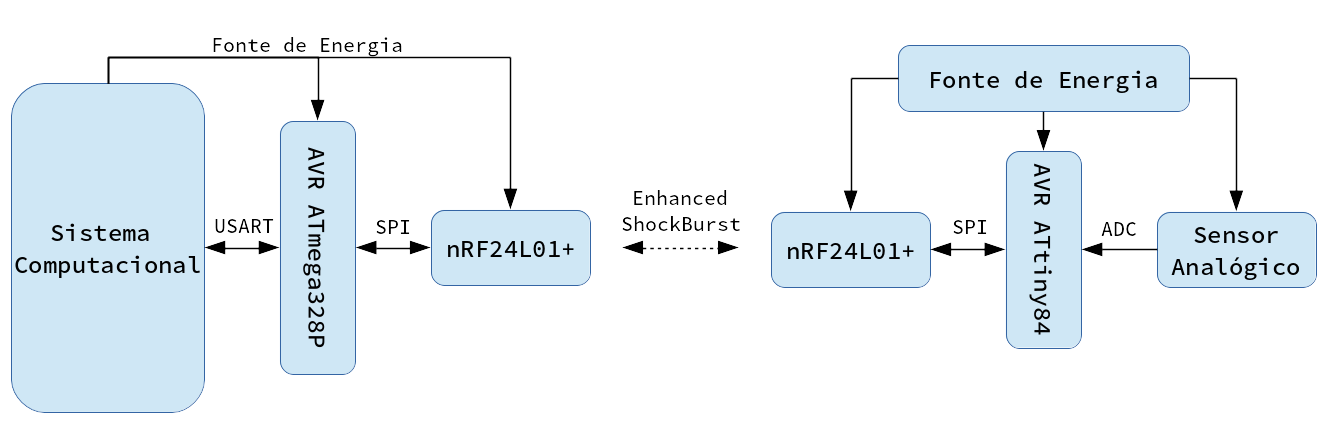
\includegraphics[width=\textwidth]{../images/diagrama_ponto_a_ponto.png}
	\hspace{\linewidth}
	Fonte: Elaborada pelo autor
	\label{figura:point_to_point}
\end{figure}

De acordo com o \textit{datasheet} do \texttt{nRF24L01+}, o tratamento da transação de pacotes entre um
dispositivo PTX ({\textit{Primary Transmitter}) e PRX (\textit{Primary Receiver}) ocorre da
seguinte maneira:

\begin{enumerate}
	\item A transação incia-se quando um pacote de dados é transmitido ao PRX. O
		\texttt{Enhanced ShockBurst} automaticamente coloca o PTX em modo de recepção para esperar
		pelo pacote de confirmação.
	\item Se o PRX receber o pacote, o \texttt{Enhanced ShockBurst} monta e transmite o pacote ACK
		(Acknowledgement) ao PTX.
	\item Se o PTX não receber o pacote ACK em um determinado tempo, ele automaticamente retransmite o
		pacote de dados. Esse processo repete-se em uma quantidade de vezes configurável ou até que o
		pacote ACK seja recebido.
\end{enumerate}

Essa transação ocorre em um uma faixa de frequência entre 2.4 GHz e 2.4835 GHz e a uma taxa de transferência
que pode ser de 250 Kbps, 1 Mbps ou 2 Mpbs que devem ser pré-definidos e iguais em ambos os
transceptores \cite{nrfdatasheet}.

Na implementação da RSSF foram definidos um tempo de espera de retranmissão de \SI{1250}{\micro \second} e uma
quantidade máxima de 15 retransmissões a uma taxa de 1 Mbps para todos os módulos. Essa configuração
permitiu uma comunicação direta a 15 metros de distância com 3 obstáculos de alvenaria no caminho e com o
Wi-Fi de rede doméstica ligado.

O formato do pacote utilizado pelo protocolo \texttt{Enhanced ShockBurst} é ilustrado na Figura
\ref{figura:package}

\begin{figure}[h!]
	\caption{Pacote \textit{Enhanced ShockBurst}}
	\centering
	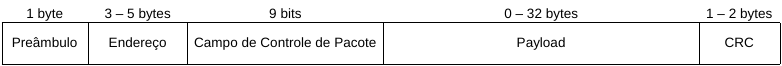
\includegraphics[scale=0.5]{../images/pacote.png}
	\hspace{\linewidth}
	Fonte: Elaborada pelo autor
	\label{figura:package}
\end{figure}

O preâmbulo é uma sequência de bits alternados usados para sincronizar o demodulador do receptor para o fluxo
de bits do pacote. O endereço, mencionado anteriormente, é anexado no pacote logo após o prêmabulo. O campo de
controle de pacote contém o tamanho do \textit{payload} utilizado, um identificador do pacote e uma flag
indicando se é necessário enviar o ACK. O \textit{payload} é onde vai o conteúdo do pacote e o tamanho
utilizado pode ser estático (pré-configurado em ambas as pontas da comunicação) ou dinâmico (utiliza a
informação sobre o tamanho contida no campo de controle). Por fim, o CRC (\textit{Cyclic Redundancy Check}) é
um mecanismo de detecção de erros no pacote \cite{nrfdatasheet}.

Tanto para transmissão como para recepção, os pacotes são enfileirados em um mecanismo de FIFO (\textit{First
In First Out}) com capacidade de até 3 pacotes. Se o FIFO de transmissão estiver cheio ao inserir um novo, o
mais antigo é descartado. Já no FIFO de recepção não é inserido um novo pacote caso o mesmo já esteja cheio.

Além disso, é possível também encapsular dados no pacote ACK, o que diminui a quantidade necessária de
transmissões em uma comunicação bi-lateral pela metade. Para isto, é necessário ativar a funcionalidade de
\textit{payload} dinâmico e deixar o pacote pronto para ser encapsulado no ACK colocando-o no FIFO de
transmissão e definindo para qual canal de recepção ele deve responder.

Portanto, para o canal de \textit{broadcast} (canal 0) o dado a ser encapsulado é o endereço do canal 1, que é o
endereço único do transceptor e para o canal 1, o dado de resposta é o valor obtido pelos sensores.

\section{Roteamento}
O protocolo de roteamento é o responsável por permitir uma comunicação indireta entre estações. Devido ao
baixo poder de processamento e baixa memória disponíveis em um MCU, o roteamento deve ser realizado de uma
maneira simples. Não é viável, por exemplo, armazenar todos os endereços das estações adjacentes nem
calcular as rotas dinamicamente como ocorre normalmente em redes de computadores.

Para atender essa necessidade, utilizou-se o próprio corpo do pacote de dados para transmitir a rota
que ele deve percorrer até o destino. Isso é possível pois o \texttt{nRF24L01+} permite até 32
\textit{bytes} de dados em seus pacotes.

Considerando que o endereço possui 5 \textit{bytes} de tamanho, 20 \textit{bytes} do \textit{payload} são
reservados para a transmissão da rota, restando 12 \textit{bytes} para a mensagem. Isso possibilita uma
comunicação indireta com até 5 saltos, pois permite com que o nó principal envie uma mensagem com uma rota de
até 4 endereços em seu \textit{payload}.

Conforme mostra a Figura \ref{figura:route}, a cada salto são retirados 5 \textit{bytes} do \textit{payload} e
utilizados como endereço do próximo salto.  Esse processo se repete até chegar ao destino, onde a mensagem é
processada. Caso ocorra alguma falha no caminho, é informado à estação principal transmitimdo o endereço em
que ela ocorreu.

\begin{figure}[h!]
	\caption{Exemplo Roteamento}
	\centering
	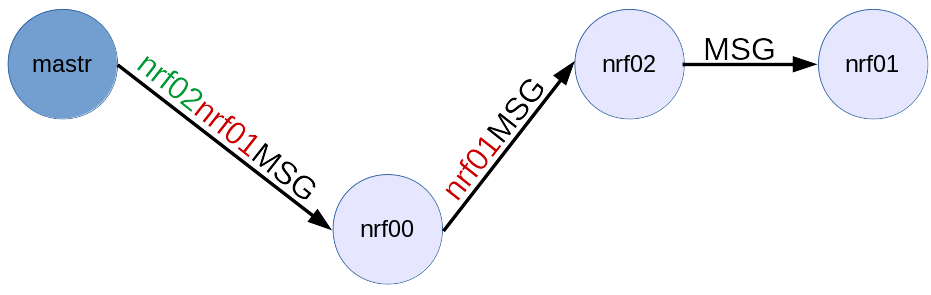
\includegraphics[scale=0.5]{../images/roteamento.png}
	\hspace{\linewidth}
	Fonte: Elaborada pelo autor
	\label{figura:route}
\end{figure}

No pior caso de uma comunicação bem-sucedida, isto é, quando a comunicação ocorre em 5 saltos com 15
retransmissões em cada um, o tempo de máximo é de aproximadamente \SI{187.5}{\milli \second}
($\SI{1250}{\micro \second} * 15 * 5 * 2$).

A única informação que os MCUs remotos precisam armazenar é o endereço da estação superior na hierarquia da
topologia da rede, ou seja, o endereço do próximo transceptor em direção à estação principal. A
responsabilidade em armazernar as rotas para todos os nós fica a cargo do sistema computacional.

\subsection{Busca do Caminho}
Ao inserir um novo nó em uma RSSF, é preciso que a estação central saiba como se comunicar com ele e
vice-versa. A maneira mais simples para fazer isso seria pré-configurar as rotas para cada estação remota.

Porém, além de ser um processo trabalhoso, dessa maneira as rotas seriam estáticas e teriam que ser
reconfiguradas manualmente toda vez que algum nó de seu percurso parasse de funcionar ou que a estação fosse
movida de posição.

Portanto, foi implementado um processo de busca por \textit{broadcast} cujo objetivo é informar ao nó
principal a existência de um novo nó e gerar a ele um endereço.

Para garantir que o um nó posicionado entre o principal e um remoto já existente tenha acesso direto ao
principal, é inicialmente realizada uma tentativa de comunicação à estação central. Se bem sucedida, o
endereço pai desse novo nó passa a ser o do próprio nó principal. Caso não obtenha resposta, significa que
está fora de seu alcance, iniciando então o processo de busca de rota por \textit{broadcast}, ilustrado na
Figura \ref{figura:broadcast}.

\begin{figure}[h!]
	\caption{Exemplo Broadcast}
	\centering
	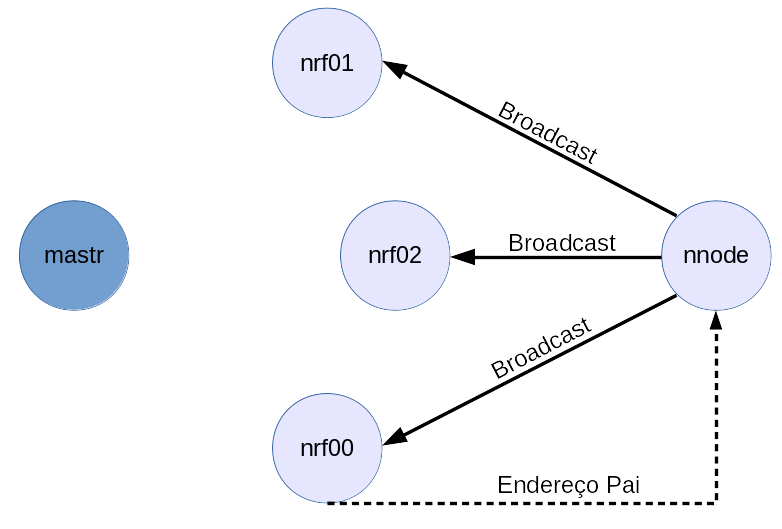
\includegraphics[scale=0.5]{../images/broadcast.png}
	\hspace{\linewidth}
	Fonte: Elaborada pelo autor
	\label{figura:broadcast}
\end{figure}

Esse processo consiste no novo nó enviar um pacote de leitura ao endereço de \textit{broadcast} da RSSF. Como
dito anteriormente, o canal do transceptor responsável pelo \textit{broadcast} envia o respectivo endereço do
próprio nó encapsulado no pacote ACK. Sendo assim, o primeiro pacote de confirmação que chegar ao novo nó
contém o endereço de seu pai na arquitetura da rede, que provavelmente é o nó mais próximo a ele, e o armazena
para futuras comunicações. Caso não receba nenhuma confirmação, porque não há algum nó em seu alcance, um LED
é ligado para alertar o fracasso.

Caso essa confirmação ocorra, é enviado o endereço atual ao nó pai, que já está localizado na rede e que, por
sua vez, anexa seu endereço no \textit{payload} de transmissão juntamente com a informação proveniente do novo
nó e envia esse pacote ao próximo nó de sua rota em direção à estação principal, conforme mostra a Figura
\ref{figura:new_route}. Esse processo se repete até que o endereço do novo nó com a rota até ele chegue no
final ou que o número de endereços anexados seja maior do que quatro, que é o máximo permitido.

\begin{figure}[h!]
	\caption{Exemplo de recebimento de uma nova rota}
	\centering
	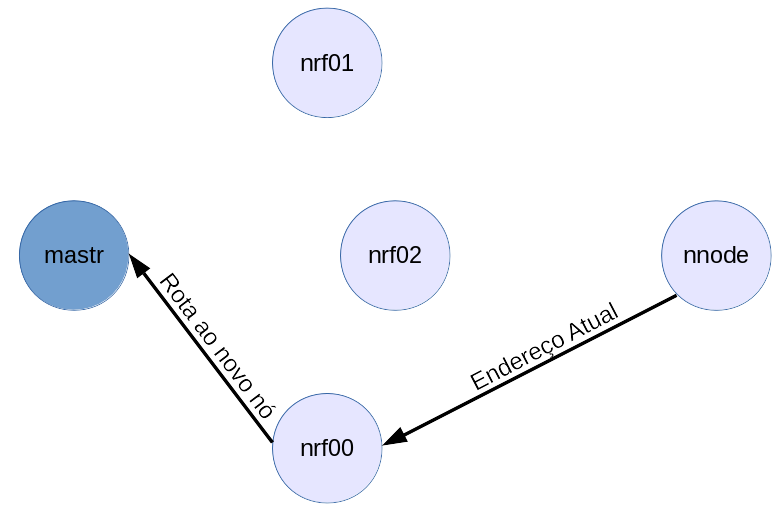
\includegraphics[scale=0.5]{../images/nova_rota.png}
	\hspace{\linewidth}
	Fonte: Elaborada pelo autor
	\label{figura:new_route}
\end{figure}

A estação central repassa a rota recebida para o computador que gera um endereço válido e que será enviado ao
novo nó para substituir o endereço padrão contido nele até então. A forma como esse endereço é gerado é
indiferente para a RSSF, contanto que não seja igual a algum já existente. Do ponto de vista de segurança, é
recomendável que ele seja gerado de forma aleatória.

Se o novo nó não receber a mensagem contendo seu novo endereço após determinado tempo, um LED é ligado para
alertar que a tentativa de ingressar na RSSF foi mal-sucedida.

\section{Mensagem}
O formato da mensagem recebida é o que determina o comportamento que a estação deve adotar naquele momento.
Sendo assim, neste capítulo será abordada a estrutura de mensagens elaborada para o desenvolvimento da RSSF
proposta.

Além de conter dados de sensores ou valores de entrada para atuadores, a mensagem também deve possuir
informações adicionais sobre os dados para que eles sejam processados de forma adequada. Foi optado por
utilizar informações a nível de \texit{byte} ao invés de \textit{bit} pois torna mais fácil a manipulação dos
dados com o custo de alguns \textit{bytes} a mais no corpo da mensagem transmitida.

Como 20 \textit{bytes} dos 32 disponíveis já estão sendo utilizados para envio da rota, as mensagens podem
possuir tamanho máximo de 12 \textit{bytes}, o que é suficiente para a implementação da RSSF, pois, como será
mostrado a seguir, a maior mensagem utilizada tem apenas 9 \textit{bytes}, deixando os 3 restantes reservados
para possíveis usos futuros.

O \textit{payload} utilizado nas comunicações que contém a mensagem é estruturado conforme ilustrado na Figura
\ref{figura:message_types}.

\begin{figure}[h!]
	\caption{Formato Geral de Mensagem}
	\centering
	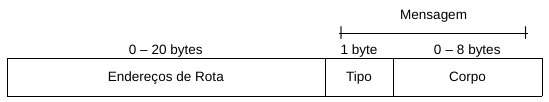
\includegraphics[scale=0.5]{../images/mensagem_tipos.png}
	\hspace{\linewidth}
	Fonte: Elaborada pelo autor
	\label{figura:message_types}
\end{figure}

O primeiro \textit{byte} da mensagem indica seu tipo, sendo 8 possíveis valores que são representados pelos
seguintes caracteres da tabela ASCII (\textit{American Standard Code for Information Interchange}):

\begin{itemize}
	\item \textbf{A:} \textit{Address} - Endereço;
	\item \textbf{E:} \textit{Emergency} - Emergência;
	\item \textbf{F:} \textit{Failure} - Falha;
	\item \textbf{M:} \textit{Measurement} - Medição;
	\item \textbf{N:} \textit{New Node} - Novo Nó;
	\item \textbf{P:} \textit{Parent} - Pai.
	\item \textbf{R:} \textit{Read} - Leitura.
	\item \textbf{W:} \textit{Write} - Escrita;
\end{itemize}

\subsection{Endereço, Falha e Pai}
Esses três tipos possuem a mesma estrutura, diferenciando-se apenas na \textit{flag} representativa do tipo,
como mostra a Figura \ref{figura:message_addr_fail_parent}.

\begin{figure}[h!]
	\caption{Mensagem do Tipo Endereço, Falha ou Pai}
	\centering
	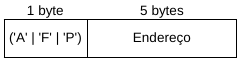
\includegraphics[scale=0.5]{../images/mensagem_end_falha_pai.png}
	\hspace{\linewidth}
	Fonte: Elaborada pelo autor
	\label{figura:message_addr_fail_parent}
\end{figure}

O valor 'A' representa um endereço gerado pelo sistema computacional e que, ao chegar ao nó de destino, é
configurado no canal de recepção 1 desse nó. O valor 'F' indica que houve uma falha ao tentar se comunicar com
aquele endereço e  é enviada à estação central quando ocorre. Já a mensagem com o tipo 'P' é a que retorna no
ACK pelo canal de \textit{broadcast}, onde o nó que a recebe armazena o endereço nela contido como seu
endereço pai na hierarquia da topologia da rede.

\subsection{Emergência}
É a única mensagem orientada à eventos, ou seja, que é enviada ao nó principal sem requisição prévia. Por
causa disso, seu endereço deve ser enviado no corpo para que o nó possa ser identificado. A estrutura é como
mostrado na Figura \ref{figura:message_emergency}.

\begin{figure}[h!]
	\caption{Mensagem do Tipo Emergência}
	\centering
	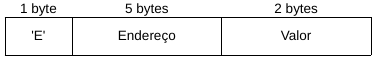
\includegraphics[scale=0.5]{../images/mensagem_emergencia.png}
	\hspace{\linewidth}
	Fonte: Elaborada pelo autor
	\label{figura:message_emergency}
\end{figure}

\subsection{Medição}
É a mensagem retornada no pacote de confirmação quando a comunicação é efetuada no canal 1. Conforme mostra
a Figura \ref{figura:message_measurement}, para cada periférico ela possui um campo que identifica o parâmetro
físico medido ou o tipo de atuador, a categoria da medição e o valor medido.

\begin{figure}[h!]
	\caption{Mensagem do Tipo Medição}
	\centering
	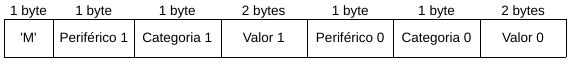
\includegraphics[scale=0.5]{../images/mensagem_medida.png}
	\hspace{\linewidth}
	Fonte: Elaborada pelo autor
	\label{figura:message_measurement}
\end{figure}

O parâmetro físico medido ou atuador são representados por um valor ASCII que é definido previamente. Os valores utilizados
por ora são 'T' (Temperatura), 'H' (umidade), 'L' (Luz), 'G' (Gás), 'R' (Relé) e '0' (Vazio). Já no campo categoria, os
valores utilizados são 'A' (Analógico) ou 'D' (Digital) e '0' quando o campo Periférico for '0'.

\subsection{Novo Nó}
É a mensagem enviada ao endereço de nó pai recebido no processo de \textit{broadcast}. Ilustrado na Figura
\ref{figura:message_new_node}, também possui campos que indicam o parâmetro ou atuador, assumindo os mesmo
valores que os campos "Periférico N`` da mensagem de medição.

\begin{figure}[h!]
	\caption{Mensagem do Tipo Novo Nó}
	\centering
	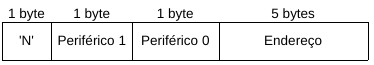
\includegraphics[scale=0.5]{../images/mensagem_novo_no.png}
	\hspace{\linewidth}
	Fonte: Elaborada pelo autor
	\label{figura:message_new_node}
\end{figure}

\subsection{Leitura}
Embora qualquer transação com um dos dois canais de recepção de um nó remoto acarrete em uma leitura, esta
mensagem, mostrada na Figura \ref{figura:message_read}, existe apenas por questão de padronização.

\begin{figure}[h!]
	\caption{Mensagem do Tipo Leitura}
	\centering
	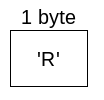
\includegraphics[scale=0.35]{../images/mensagem_leitura.png}
	\hspace{\linewidth}
	Fonte: Elaborada pelo autor
	\label{figura:message_read}
\end{figure}

\subsection{Escrita}
É o tipo de mensagem utilizado para escrever valores aos periféricos, indicada na Figura
\ref{figura:message_esc}.

\begin{figure}[h!]
	\caption{Mensagem do Tipo Escrita}
	\centering
	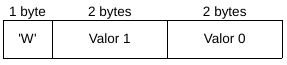
\includegraphics[scale=0.5]{../images/mensagem_escrita.png}
	\hspace{\linewidth}
	Fonte: Elaborada pelo autor
	\label{figura:message_esc}
\end{figure}

O valor contido é diretamente o que será transmitido ao atuador. Caso o periférico em questão seja
um sensor, o valor é ignorado.

\section{Experimentação}
Para experimento foram utilizados cinco estações, onde uma delas é a principal e as demais remotas. Os
transdutores foram selecionados de modo que se possa explorar todas as características da implementação da
RSSF, sendo eles:

\begin{itemize}
	\item Fotoresistor: para operar com valores analógicos;
	\item Temperatura e Umidade Digitais: para ter uma estação com dois periféricos;
	\item Relé Eletromecânico: um atuador para utilizar a mensagem de comando;
	\item Sensor de Gás: um sensor de emergência para testar a orientação à evento.
\end{itemize}

A comunicação entre o computador e o nó central foi realizada através do programa \texttt{CuteCom}, mostrado na Figura
\ref{figura:cutecom}.

\begin{figure}[h!]
	\caption{CuteCom}
	\centering
	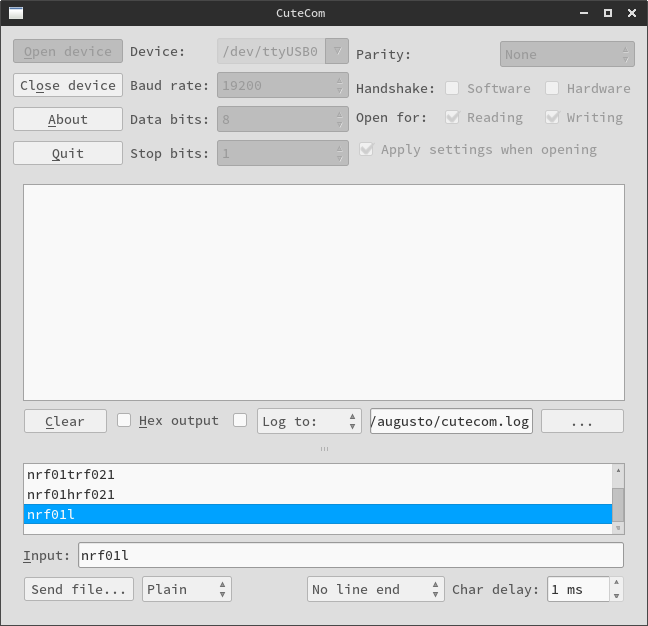
\includegraphics[scale=0.35]{../images/cutecom.png}
	\hspace{\linewidth}
	Fonte: Elaborada pelo autor
	\label{figura:cutecom}
\end{figure}

\subsection{Protótipos}
Como a estação principal utiliza USART para se comunicar com o sistema computacional, o MCU utilizado
precisa ter essa funcionalidade, sendo utilizado então o ATmega328P como mostra a figura
\ref{figura:prot_main}. Para possibilitar a comunicação USART é utilizado um dispositivo conversor USB/Serial,
que também atua como fonte de energia ao MCU e ao transceptor, que suporta até 3.3 V.

\begin{figure}[H]
	\caption{Protótipo Estação Principal}
	\centering
	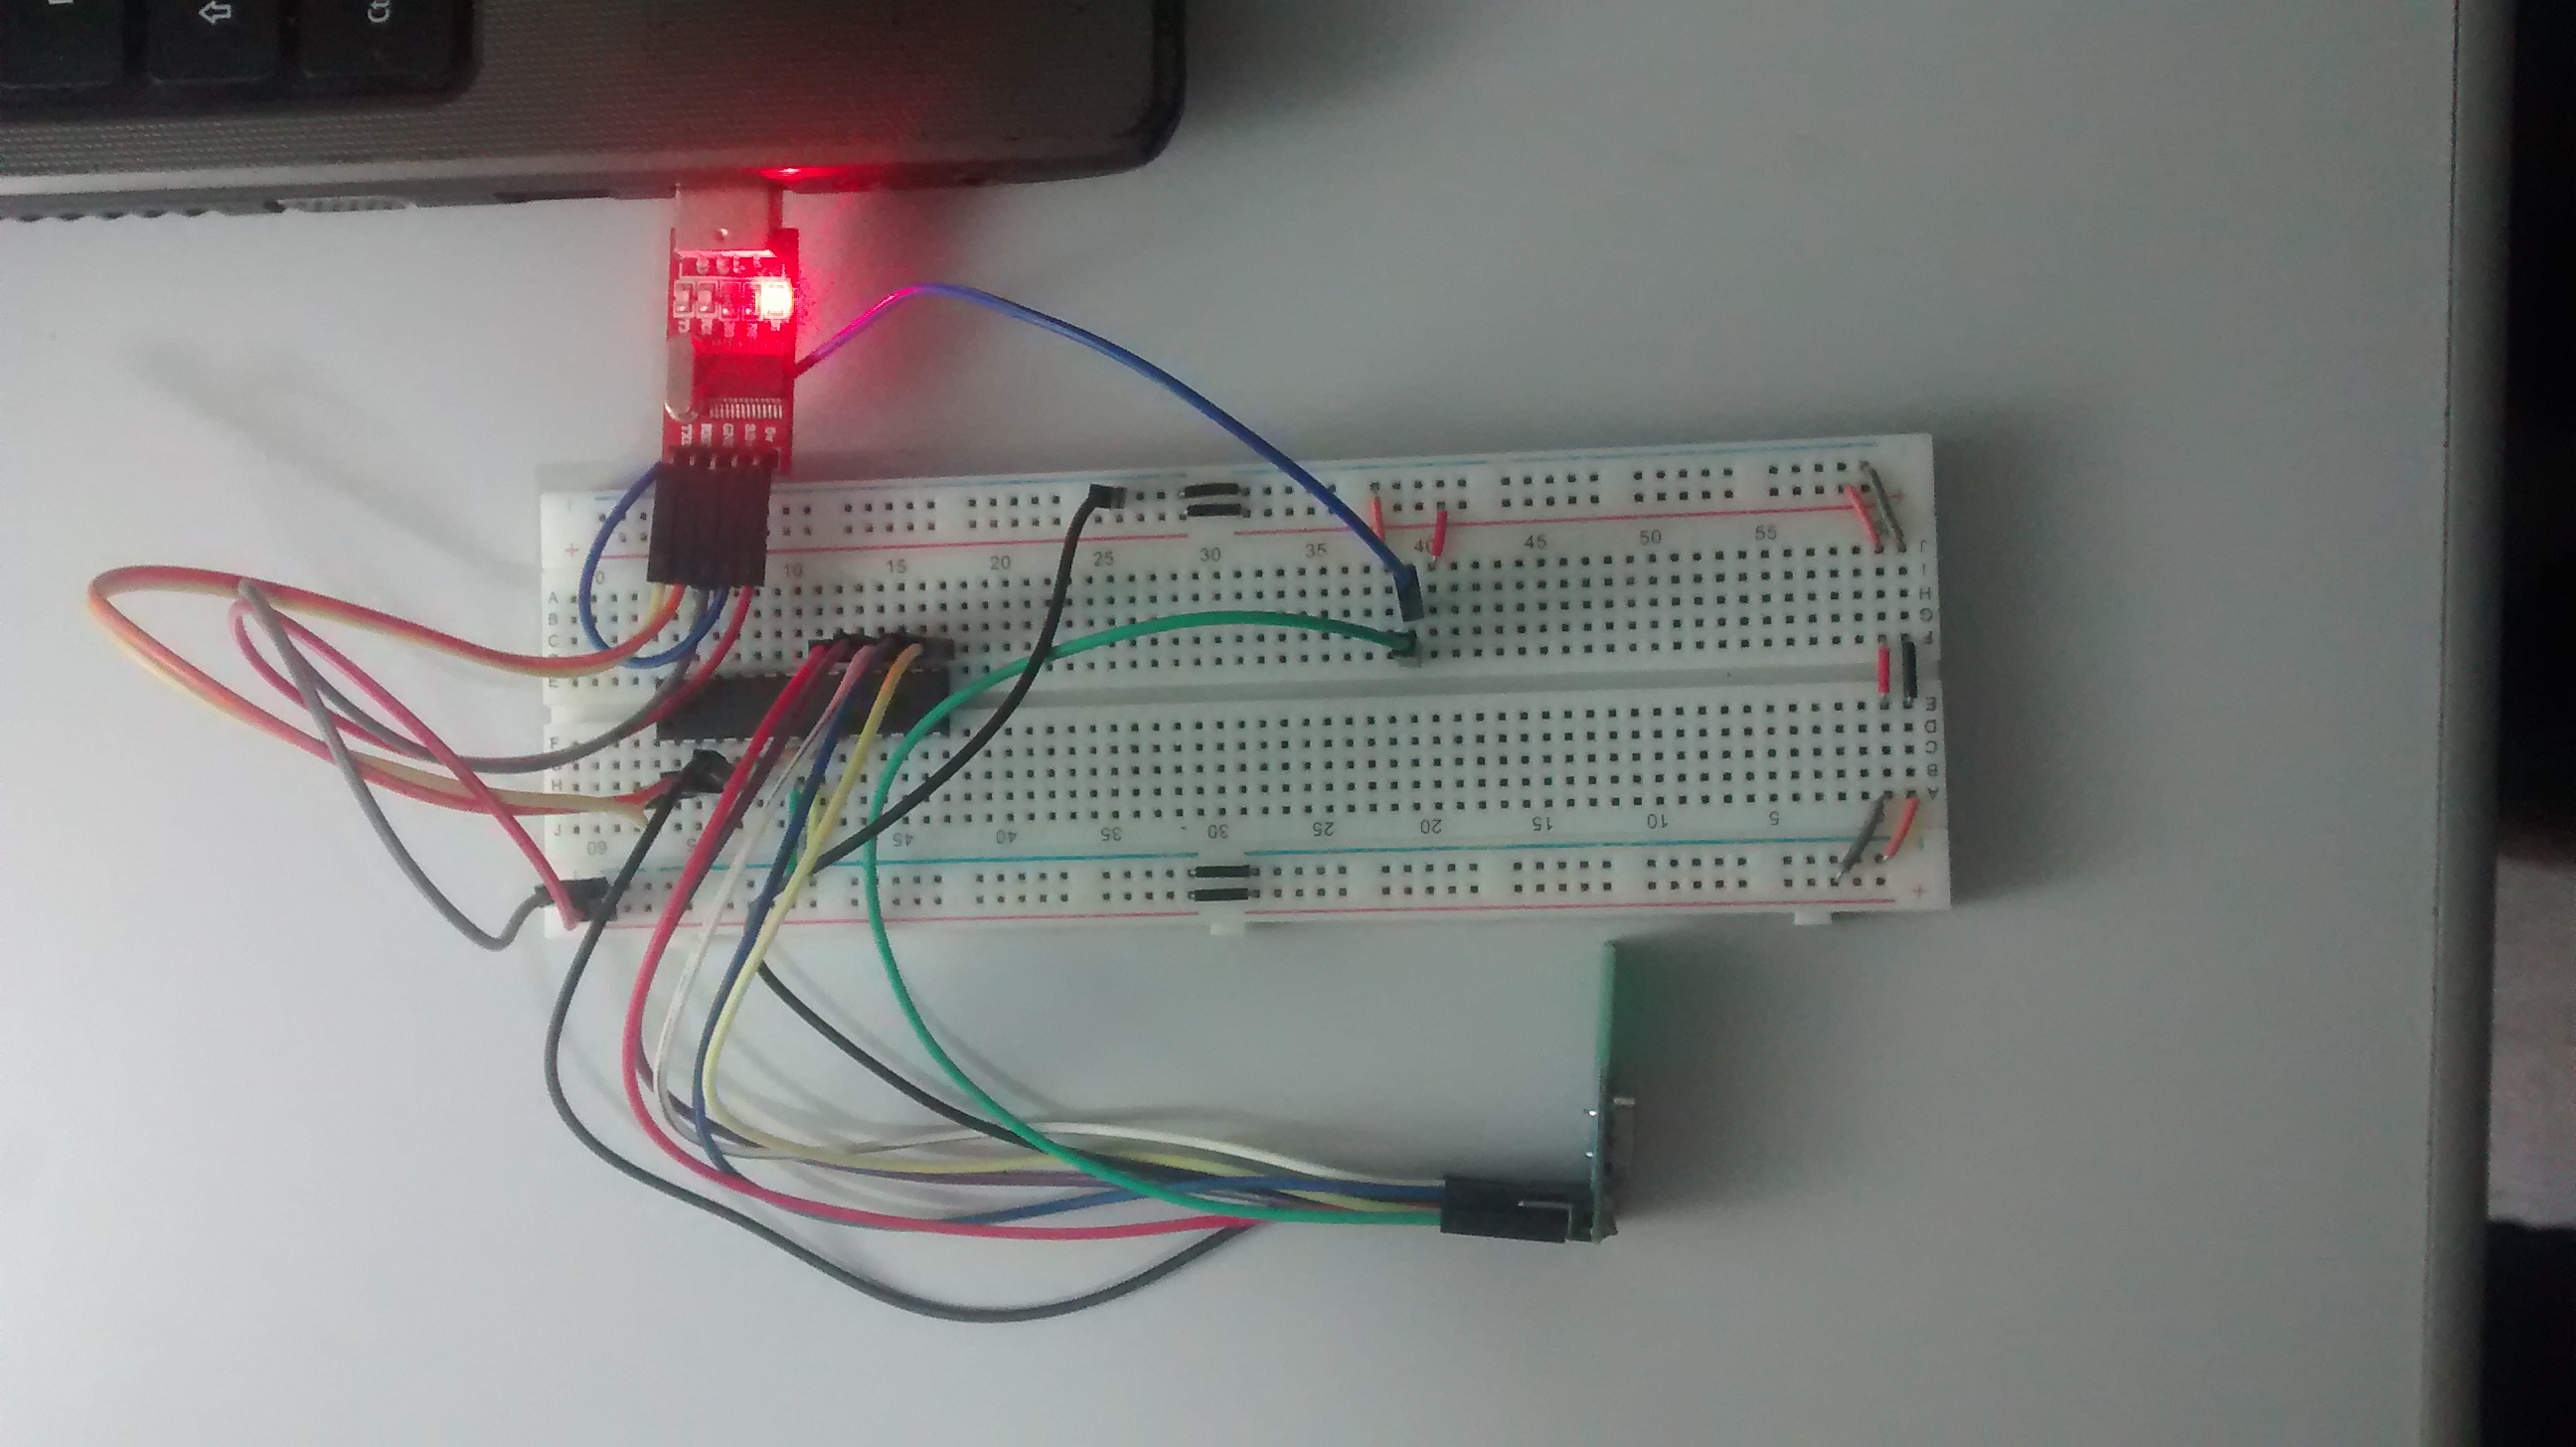
\includegraphics[scale=0.1]{../images/prot_principal.jpg}
	\hspace{\linewidth}
	Fonte: Elaborada pelo autor
	\label{figura:prot_main}
\end{figure}

Já os nós remotos não precisam de USART, tornando possível utilizar MCUs mais simples como o ATtiny84. A
Figura \ref{figura:prot_remote} exemplifica um protótipo de nó remoto contendo um sensor digital de umidade e
temperatura. O LED à direita é utilizado para sinalizar que o ingresso na rede falhou e à esquerda do sensor
há um circuito conversor de tensão usado para gerar uma tensão de 3.3 V necessária para alimentar o transceptor.

\begin{figure}[H]
	\caption{Protótipo Estação Remota}
	\centering
	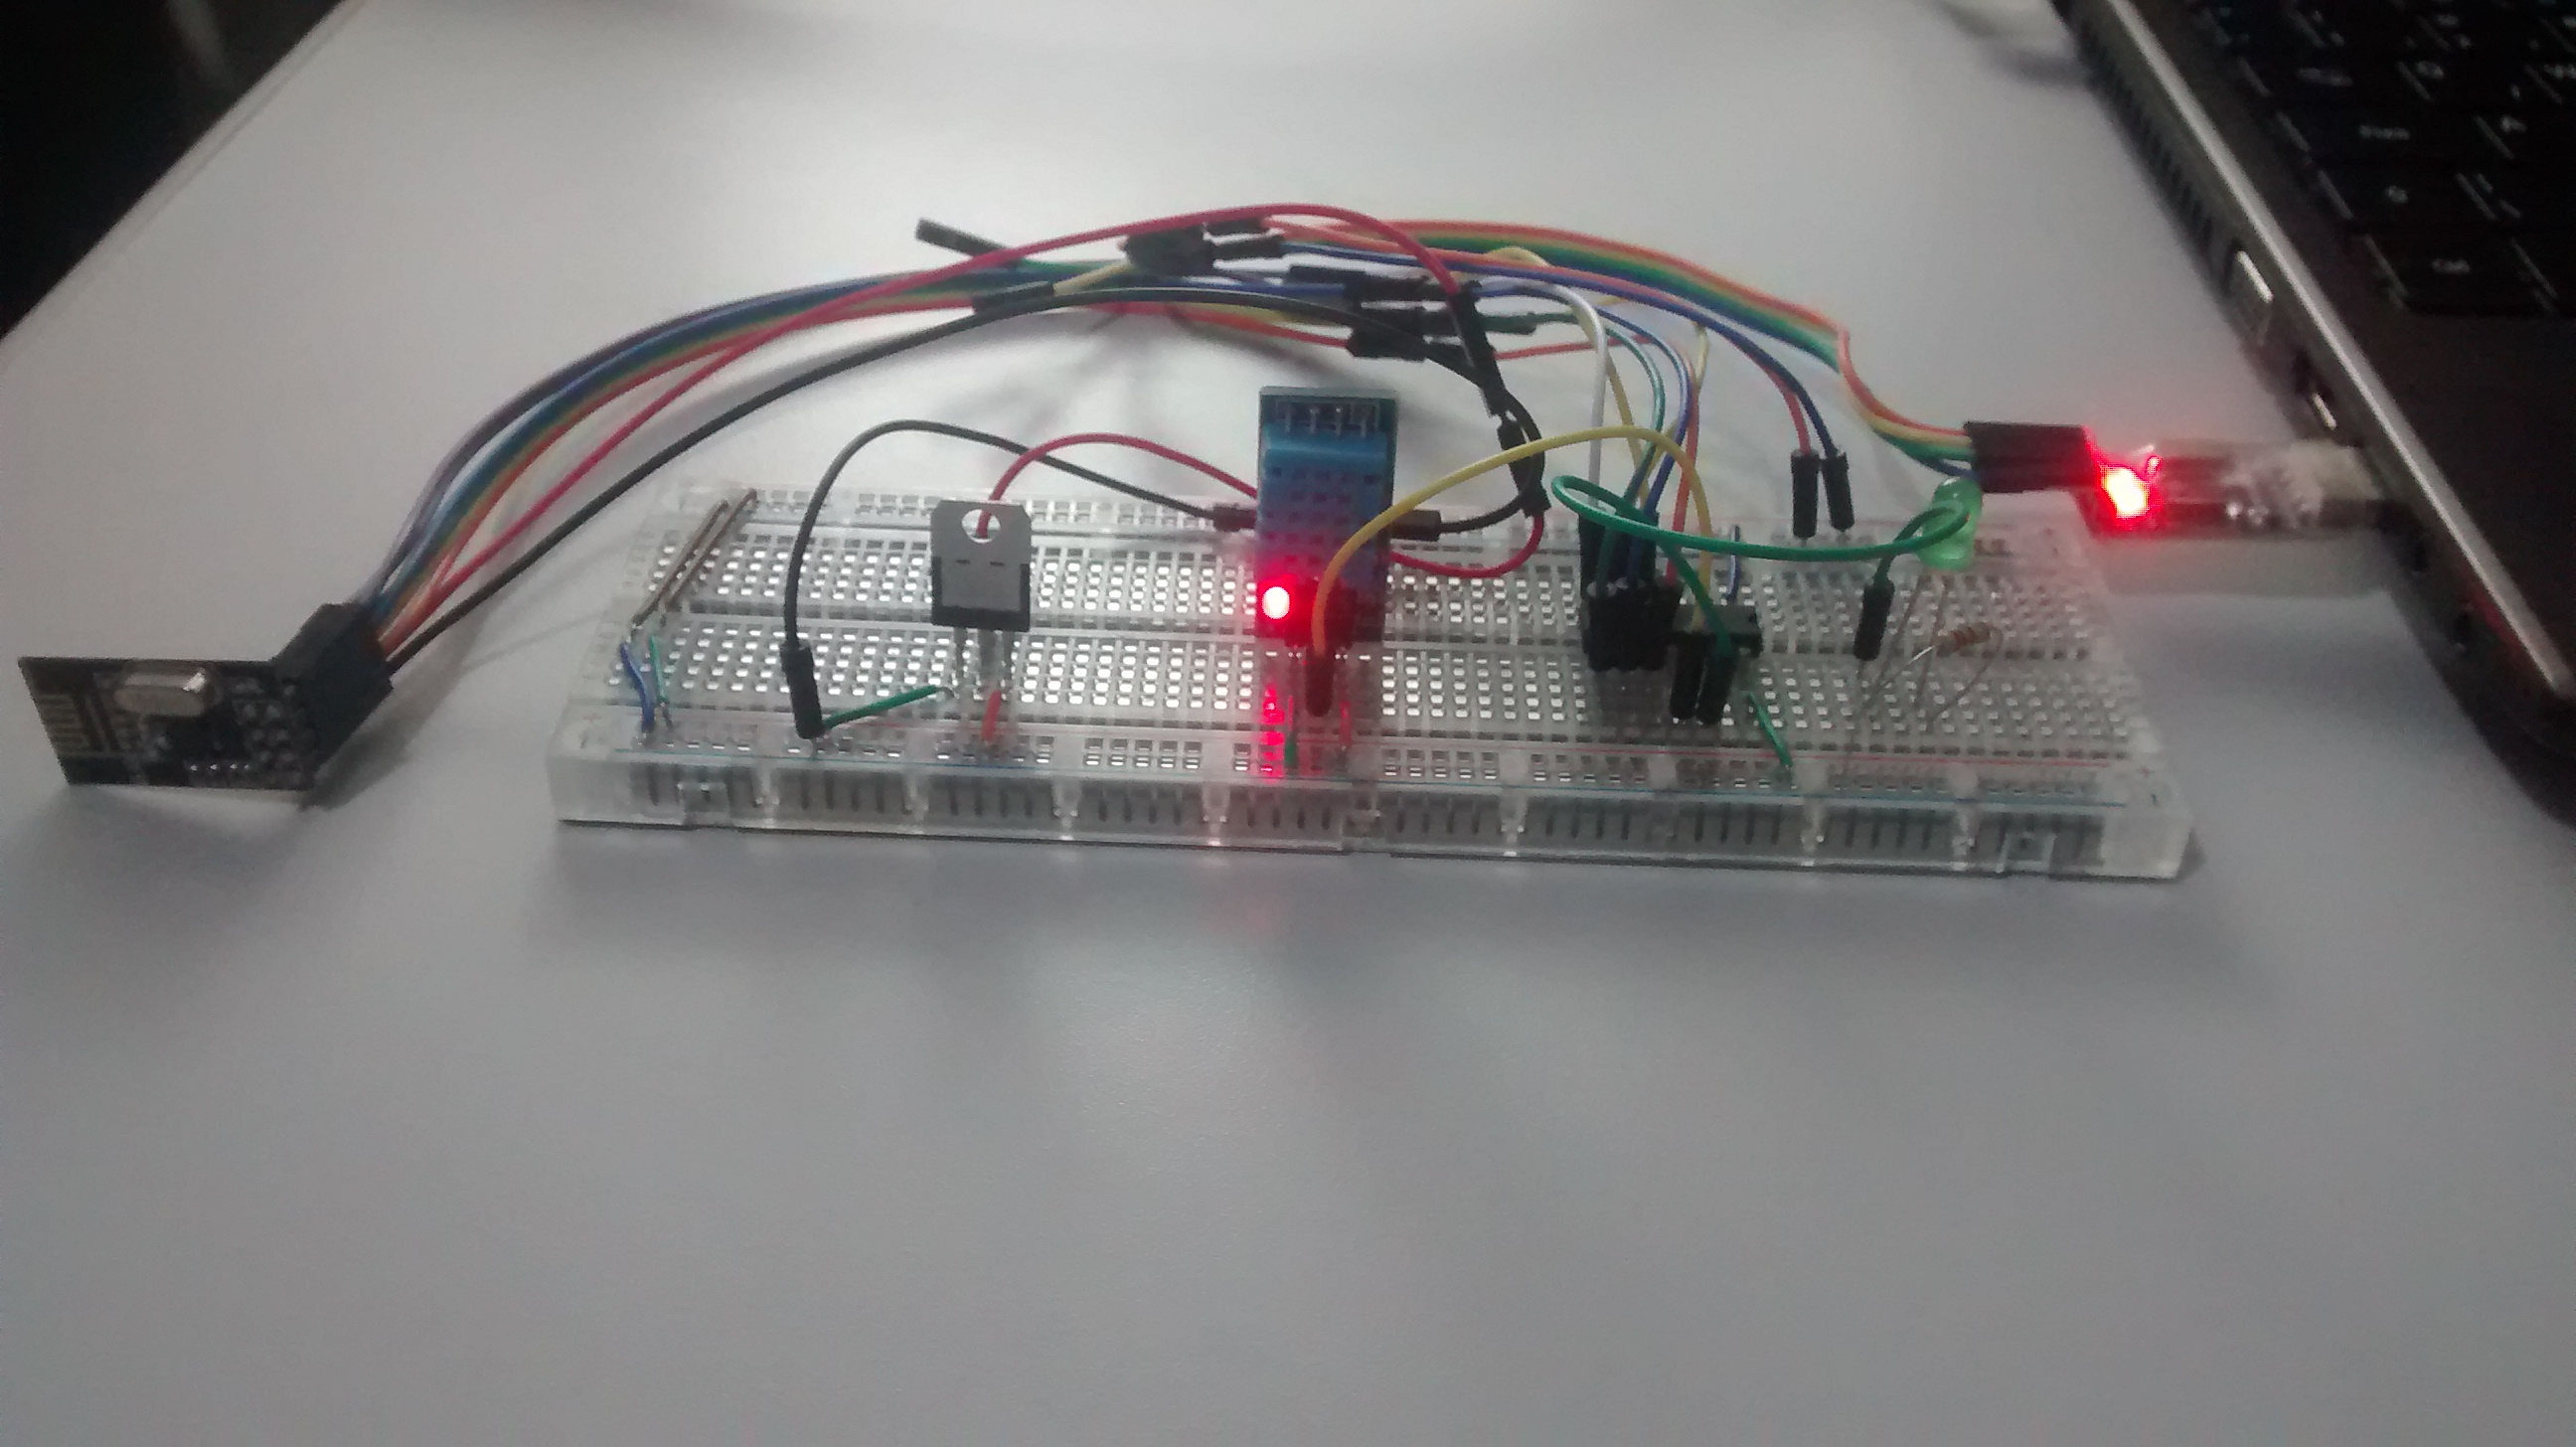
\includegraphics[scale=0.1]{../images/prot_remoto.jpg}
	\hspace{\linewidth}
	Fonte: Elaborada pelo autor
	\label{figura:prot_remote}
\end{figure}

\subsection{Testes}
Primeiramente foram realizados testes de comunicação ponto a ponto. Nesta etapa houve um contra-tempo pois
alguns erros esporádicos estavam ocorrendo. Uma leitura completa ao \textit{datasheet} do transceptor permitiu
identificar e corrigir esses erros, que estavam relacionados ao tempo de espera necessário para mudar de um
estado ao outro, à necessidade de restaurar as \textit{flags} de interrupções e à limpeza de buffer.

Após essa fase, elaborou-se como a RSSF se comportaria, sendo definidos então a estrutura das mensagens, a
taxa de transferência, número de retransmissões automáticas, entre outros quesitos também já mencionados
anteriormente neste capítulo.

A Tabela \ref{quadro:test_route} exibe o resultado do processo de inserção de nós na rede, onde cada módulo
transmitiu seu endereço padrão (nnode), tal como a identificação de seu(s) transdutor(es). Os endereços foram
gerados pelo nó principal e de forma sequencial apenas para fins de teste.

\begin{table}[H]
	\centering
	\begin{tabular}{|l|c|c|c|}
		\hline
		\textbf{Nó}           & \textbf{Mensagem Novo Nó} & \textbf{Rota} & \textbf{Endereço Recebido} \\ \hline
		Luz                   & NL0nnode & \text{\textbf{---}} & nrf00 \\ \hline
		Temperatura e Umidade & NTHnnode & \text{\textbf{---}} & nrf01 \\ \hline
		Gás                   & NG0nnode & \text{\textbf{---}} & nrf02 \\ \hline
		Relé Eletromecânico   & NR0nnode & nrf02         & nrf03       \\ \hline
	\end{tabular}
	\caption{Processo de roteamento testado}
	\label{quadro:test_route}
\end{table}

Na Tabela \ref{quadro:sample_tests} são expostos os resultados de alguns testes realizados com a solução
desenvolvida. Os trechos fora das aspas nas mensagens recebidas correspondem aos valores obtidos pelos
sensores já convertidos para um tipo numérico de dados. Após realizar os testes de leitura e escrita aos nós,
foi feita uma exposição de gás butano ao sensor de gás, gerando um pacote de emergência após atingir um
valor limiar definido como 300.

Em seguida, testou-se uma comunicação de 4 saltos entre o nó principal e o nó de luz. Embora o roteamento para
o mesmo tenha sido obtido de forma direta, isto foi possível devido à ausência de um sistema computacional que
gerencia as rotas, feitas de forma manual durante os testes. Por fim, foi realizada uma tentativa de
comunicação com um endereço inexistente, gerando assim um pacote que indica a ocorrência de falha.

\begin{table}[H]
	\centering
	\resizebox{\textwidth}{!}{%
		\begin{tabular}{|l|c|c|c|c|}
			\hline
			\textbf{Descrição}                                                         & \textbf{Destinatário} & \textbf{Rota}   & \textbf{Mensagem Enviada} & \textbf{Mensagem Recebida} \\ \hline
			Leitura Nó Luz                                                             & nrf00                 & \text{---}      & “R”                       & “MLA” 675 “00” 0           \\ \hline
			\begin{tabular}[c]{@{}l@{}}Leitura Nó Temperatura\\ e Umidade\end{tabular} & nrf01                 & \text{---}      & “R”                       & “MTD” 25 “HD” 67           \\ \hline
			Leitura Nó Gás                                                             & nrf02                 & \text{---}      & “R”                       & “MGA” 123 “00” 0           \\ \hline
			Escrita Nó Relé                                                            & nrf03                 & nrf02           & “W10”                     & \text{---}                 \\ \hline
			\begin{tabular}[c]{@{}l@{}}Emergência Nó Gás\\ (Limiar = 300)\end{tabular} & \text{---}            & \text{---}      & \text{---}                & “Enrf02” 305               \\ \hline
			Teste Múltiplos Saltos                                                     & nrf00                 & nrf02nrf03nrf01 & “R”                       & “MLA” 678 “00” 0           \\ \hline
			Teste Endereço Inexistente                                                 & nrf04                 & nrf00nrf01      & “R”                       & “Fnrf04”                   \\ \hline
		\end{tabular}%
	}
	\caption{Exemplos de testes realizados}
	\label{quadro:sample_tests}
\end{table}

\section{Custo e Consumo}
Considerando uma casa de 10 cômodos, onde cada um possui um nó para temperatura e umidade, um para luz e uma
para relé. E ainda considerando um nó para sensor de gás na cozinha, cinco nós de sensor de umidade em sólidos
para plantas e um principal, a quantidade total de nós seria igual a 37.

A Tabela \ref{quadro:compare} baseia-se nessa quantidade para comparar a solução obtida com uma solução
utilizando um \texttt{Arduino Mini} como MCU e um \textit{XBee} como transceptor, que é a configuração
normalmente utilizada em implementações caseiras encontradas na \textit{Internet}. Os preços dos sensores e
atuadores não estão sendo levados em consideração pois são constantes, ou seja, independem da implementação
utilizada.

\begin{table}[H]
	\centering
	\resizebox{\textwidth}{!} {
		\begin{tabular}{l|c|c|c|c|c|}
		\cline{2-6}
		& MCU & Transceptor & Nó Principal & Nó Remoto & Total \\ \hline
		\multicolumn{1}{|l|}{Solução Obtida} & U\$ 3,70 / U\$ 1,80 & U\$ 1,00    & U\$ 4,70     & U\$
		2,80  & U\$ 105,50    \\ \hline
		\multicolumn{1}{|l|}{Solução Comum}  & U\$ 10,00         & U\$ 25,00   & U\$ 35,00    & U\$ 35,00 & U\$ 1.295,00 \\ \hline
		\end{tabular}
	}
	\caption{Comparação entre implementações de RSSF}
	\label{quadro:compare}
\end{table}

Quanto ao alcance, é possível cobrir uma área com raio de até 50 metros com obstáculos no interior. Isso
permite instalar a RSSF em uma residência com 500 $m^2$ (50x10), por exemplo. Em relação ao consumo elétrico,
o nRF24L01+ é o transceptor com maior eficiência conforme mostrado na Tabela \ref{quadro:transceivers} do
Capítulo \ref{cap:4} e é o fator determinante neste quesito, já que a diferença de consumo entre os
microcontroladores é muito pequena.

\section{Considerações Finais}
O resultado obtido nesta etapa é fruto de um estudo detalhado de várias características dos
microcontroladores \texttt{AVR} tal como do funcionamento do módulo transceptor \texttt{nRF24L01+}.

Embora a solução obtida não possua uma característica totalmente \textit{plug-and-play}, a quantidade de
configuração necessária é mínima, sendo ela a definição dos endereços da estação principal e de
\textit{broadcast} da RSSF.
